\documentclass[10pt,a4paper]{article}
\usepackage[utf8x]{inputenc}
\usepackage{ucs}
\usepackage[MeX]{polski}
\usepackage{fancyhdr}
\usepackage{amsmath}
\usepackage{amsfonts}
\usepackage{amssymb}
\pagestyle{fancy}
\usepackage{enumerate}
\usepackage{listings}
\usepackage{subfig}
\usepackage[final]{pdfpages}

\begin{document}
\begin{figure}[!htb]
\centering

\includegraphics[scale=1.6]{logo.png}
\end{figure}
\LARGE\centering Założenia projektowe\\
\large\centering Projekt realizowany w ramach kursu Wizualizacja Danych Sensorycznych na Politechnice Wrocławskiej\\
\vspace{5 mm}
\normalsize\flushleft\textbf{Tytuł Projektu:} Wizualizacja czujników rękawicy sensorycznej\\
\textbf{Autorzy:} Krzysztof Dąbek 218549, Dymitr Choroszczak 218627\\
\textbf{Kierunek:} Automatyka i Robotyka\\
\textbf{Specjalność:} Robotyka (ARR)\\
\textbf{Prowadzący:} dr inż. Bogdan Kreczmer\\
\textbf{Kurs:} Wizualizacja Danych Sensorycznych\\
\textbf{Termin zajęć:} pt 11:15\\
\vspace{5 mm}

\section{Opis projektu} \normalsize
\subsection{Cele projektu}
Celem jest wizualizacja uproszczonego modelu dłoni na podstawie danych z rękawicy sensorycznej. 
Efektem końcowym jest przedstawienie orientacji dłoni oraz zgięcia palców w przestrzeni trójwymiarowej. \\

\subsection{Problem projektu}
\begin{itemize}
\item Ukazanie zgięcia pięciu palców przez zmianę konfiguracji przegubów modelu
\item Ukazanie siły nacisku opuszków na powierzchnię poprzez zmianę koloru i/lub rozmiaru obiektów sferycznych, umieszczonych na zakończeniach skrajnych przegubów modelu
\item Ukazanie orientacji dłoni względem wektora grawitacji
\end{itemize}

Projekt zostanie połączony z innym realizowanym w ramach kursu Roboty Mobilne 1. Dane do wizualizacji będą wysyłane przez płytkę wykonanej rękawicy sensorycznej.

\section{Specyfikacja aplikacji}

\subsection{Funkcjonalności aplikacji}
Zostanie stworzona aplikacja okienkowa do wizualizacji napisana w języku C++ z użyciem biblioteki Qt.\\
\begin{itemize}
\item Wizualizacja poruszania modelem dłoni na podstawie odczytów z czujników i akcelerometru.
\item Wybór opcji połączenia z rękawicą sensoryczną (Bluetooth, USB, UART)
\item Uruchomienie i zatrzymanie pomiarów, wykonanie pojedynczego pomiaru.
\item Skalowanie modelu dłoni poprzez wpisanie rozmiarów oraz suwak.
\item Zmiana położenia i orientacji kamery z poziomu interfejsu graficznego.
\item Zmiana rotacji modelu dłoni (RPY) poprzez suwaki interfejsu graficznego.
\item Wyświetlanie liczbowo wyników pomiarów i możliwość zapisania ich do pliku.
\item Wyświetlenie dynamicznego wykresu odczytu nacisku wybranego palca w czasie.
\end{itemize}
Wszystkie funkcjonalności zostały zaimplementowane. Zrezygnowano z połączenia przez Bluetooth z powodu braku działającego modułu Bluetooth na komputerze oraz niezadowalającej prędkości przesyłania.

\newpage
\subsection{Interfejs graficzny}
Schematyczny szkic interfejsu graficznego został przedstawiony na rysunku \ref{fig:interface}.
\begin{figure}[!htb]
\centering
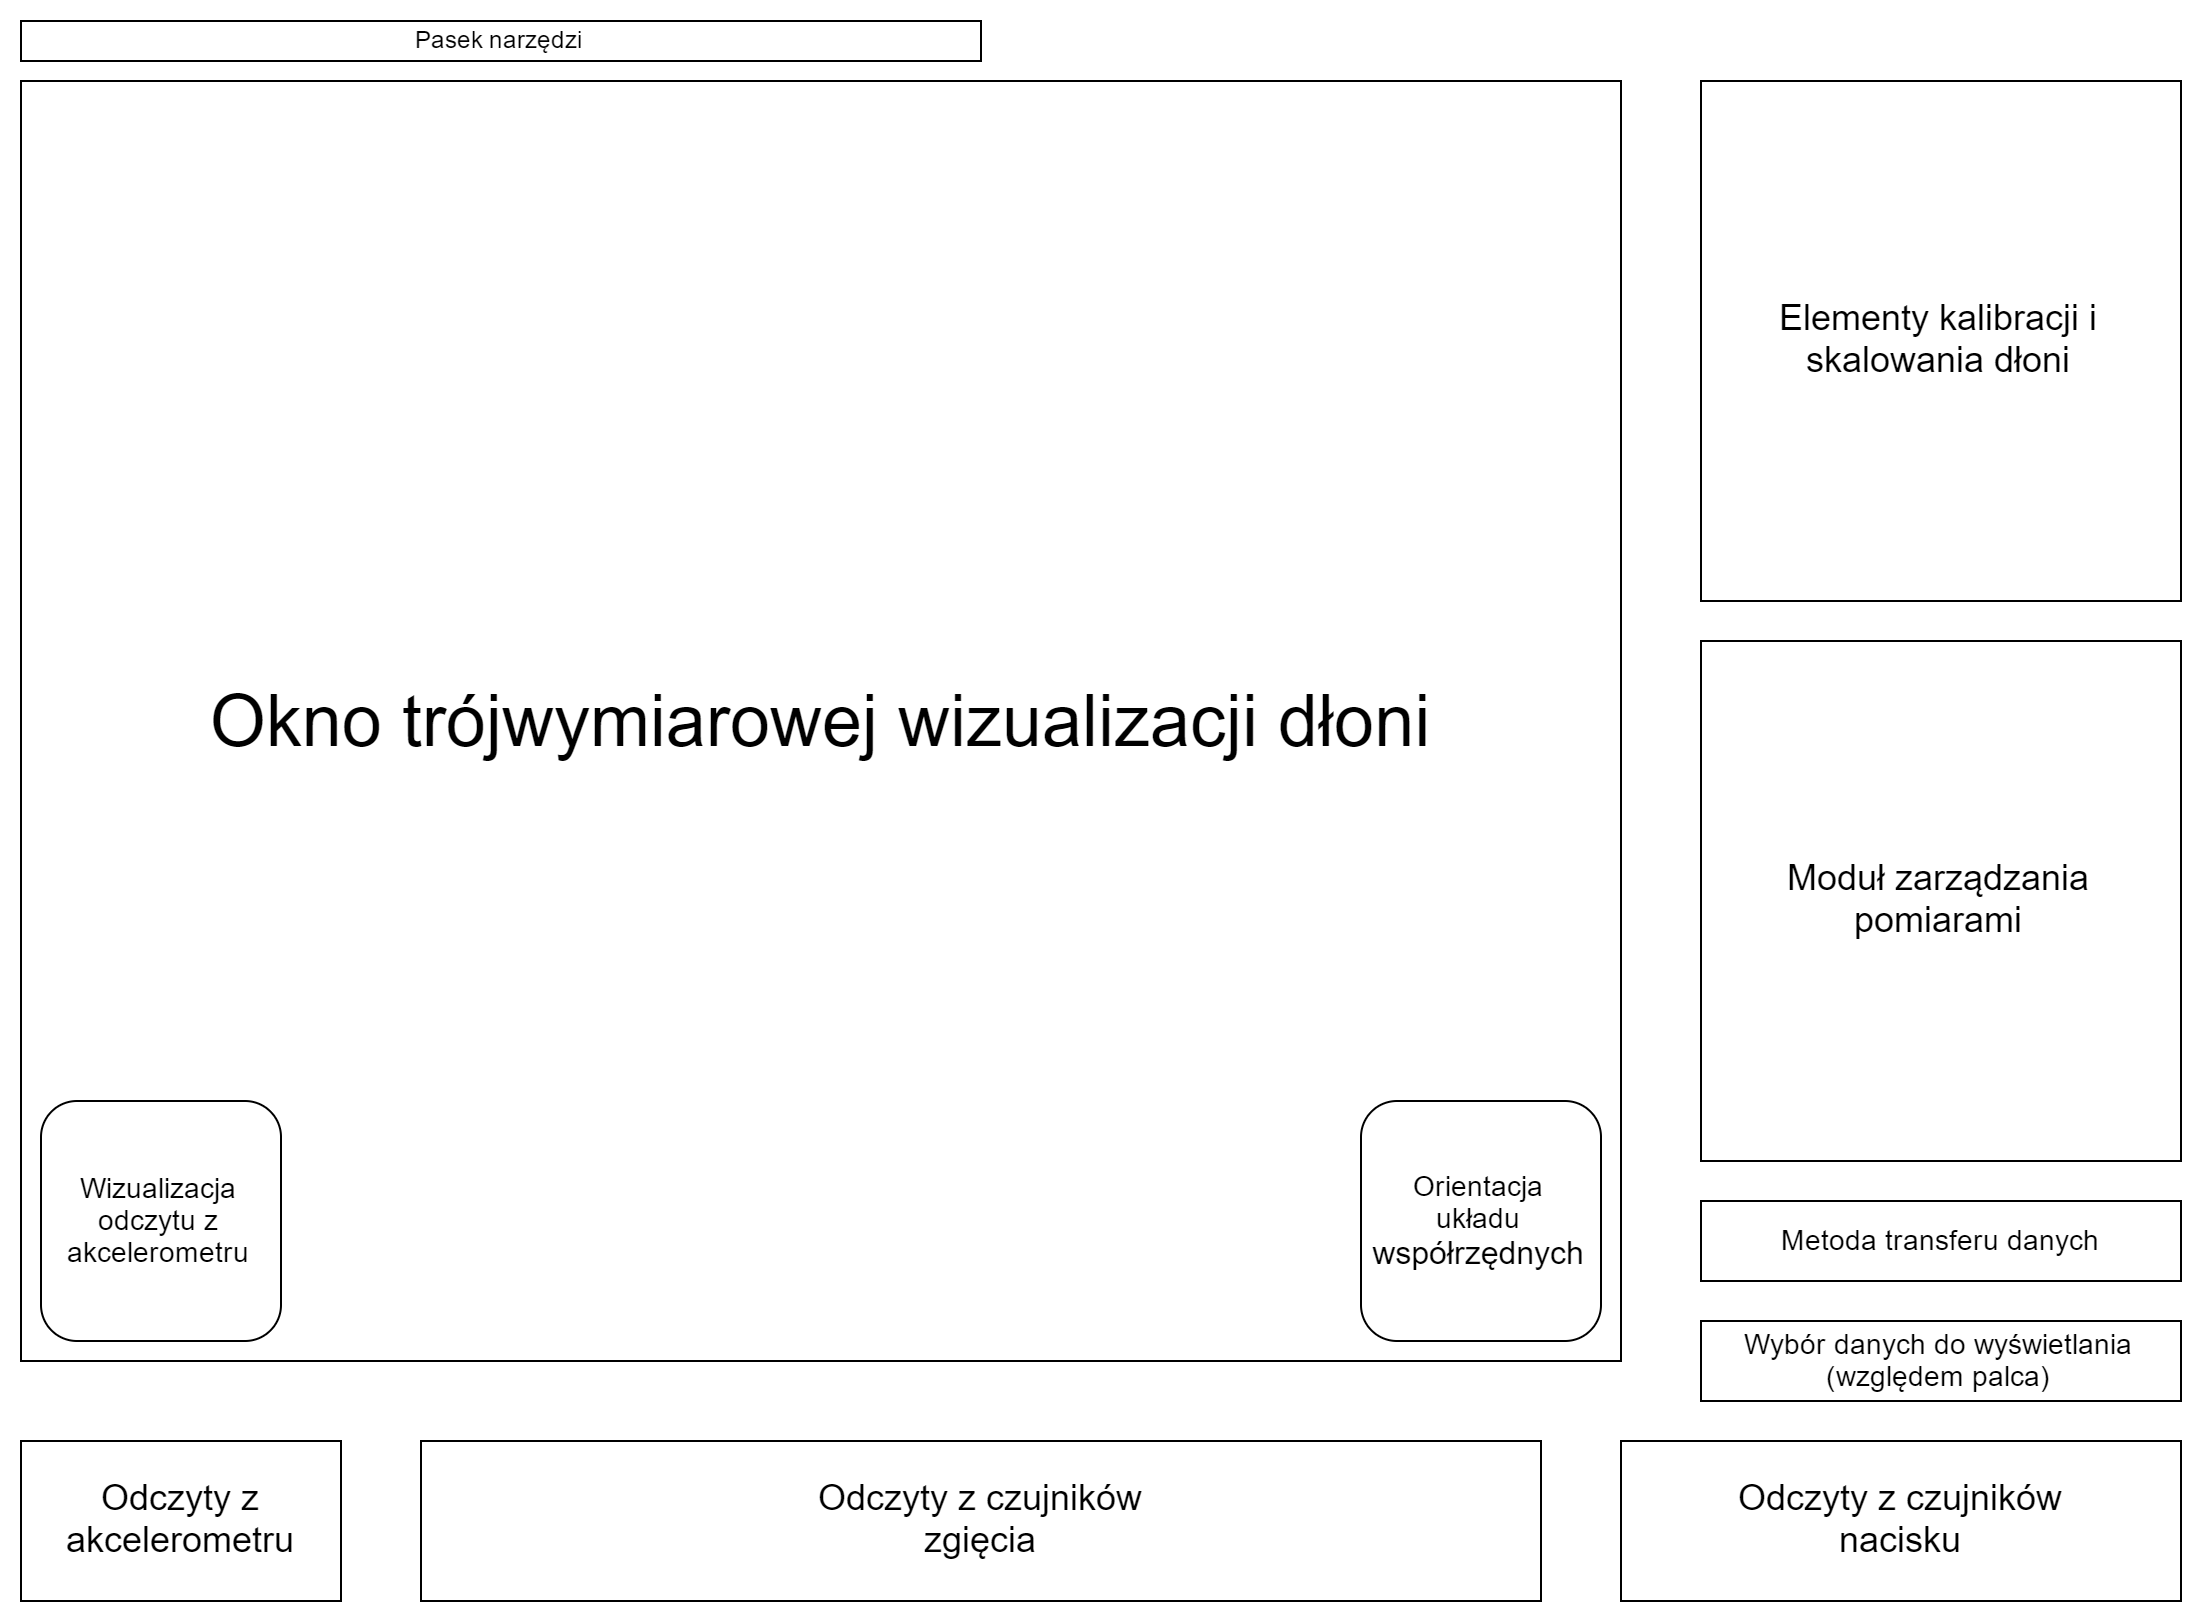
\includegraphics[width=0.9\textwidth]{./WDS_schemat_ideowy_okna_programu.png}
\caption{Planowany interfejs graficzny aplikacji\label{fig:interface}}
\end{figure}\\
\newpage
Aktualny interfejs graficzny został przedstawiony na rysunkach \ref{fig:currentInt} i \ref{fig:currentIntChart}.
\begin{figure}[!htb]
\centering
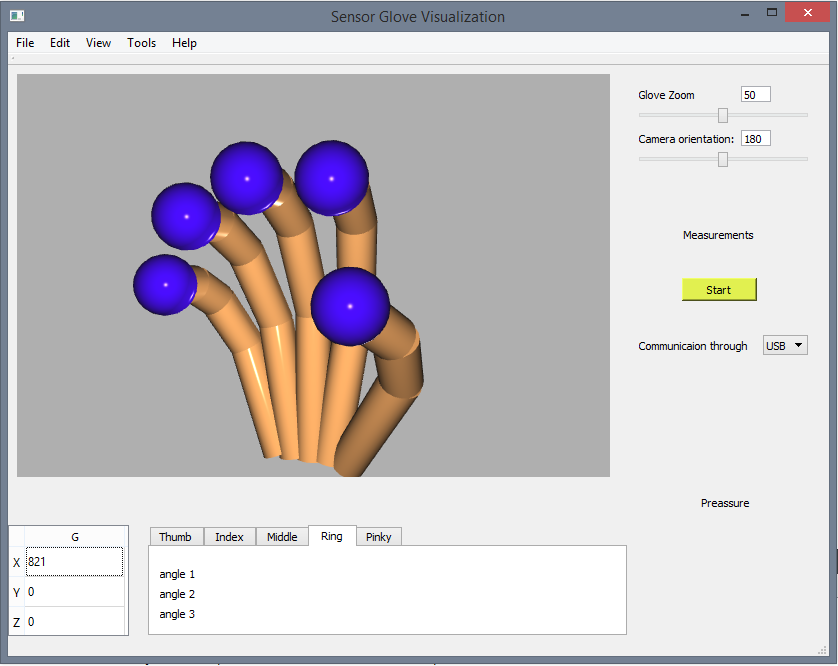
\includegraphics[width=0.9\textwidth]{./AktualnyInterfejsGraficzny.png}
\caption{Aktualny wygląd interfejsu graficznego aplikacji\label{fig:currentInt}}
\end{figure}
\begin{figure}[!htb]
\centering
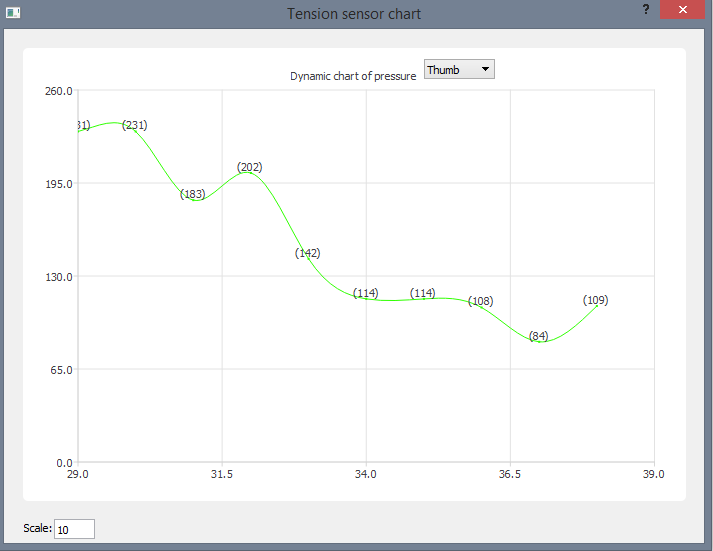
\includegraphics[width=0.9\textwidth]{./AktualnyInterfejsGraficznyChart.png}
\caption{Aktualny wygląd interfejsu graficznego aplikacji (wykresy)\label{fig:currentIntChart}}
\end{figure}

\newpage
\subsection{Diagram klas}
Diagram klas przetwarzających dane i obliczeniowych w aplikacji, przedstawiony na rysunku \ref{fig:classdiagram} wykonany został w języku UML.\\
\begin{figure}[!htb]
\centering
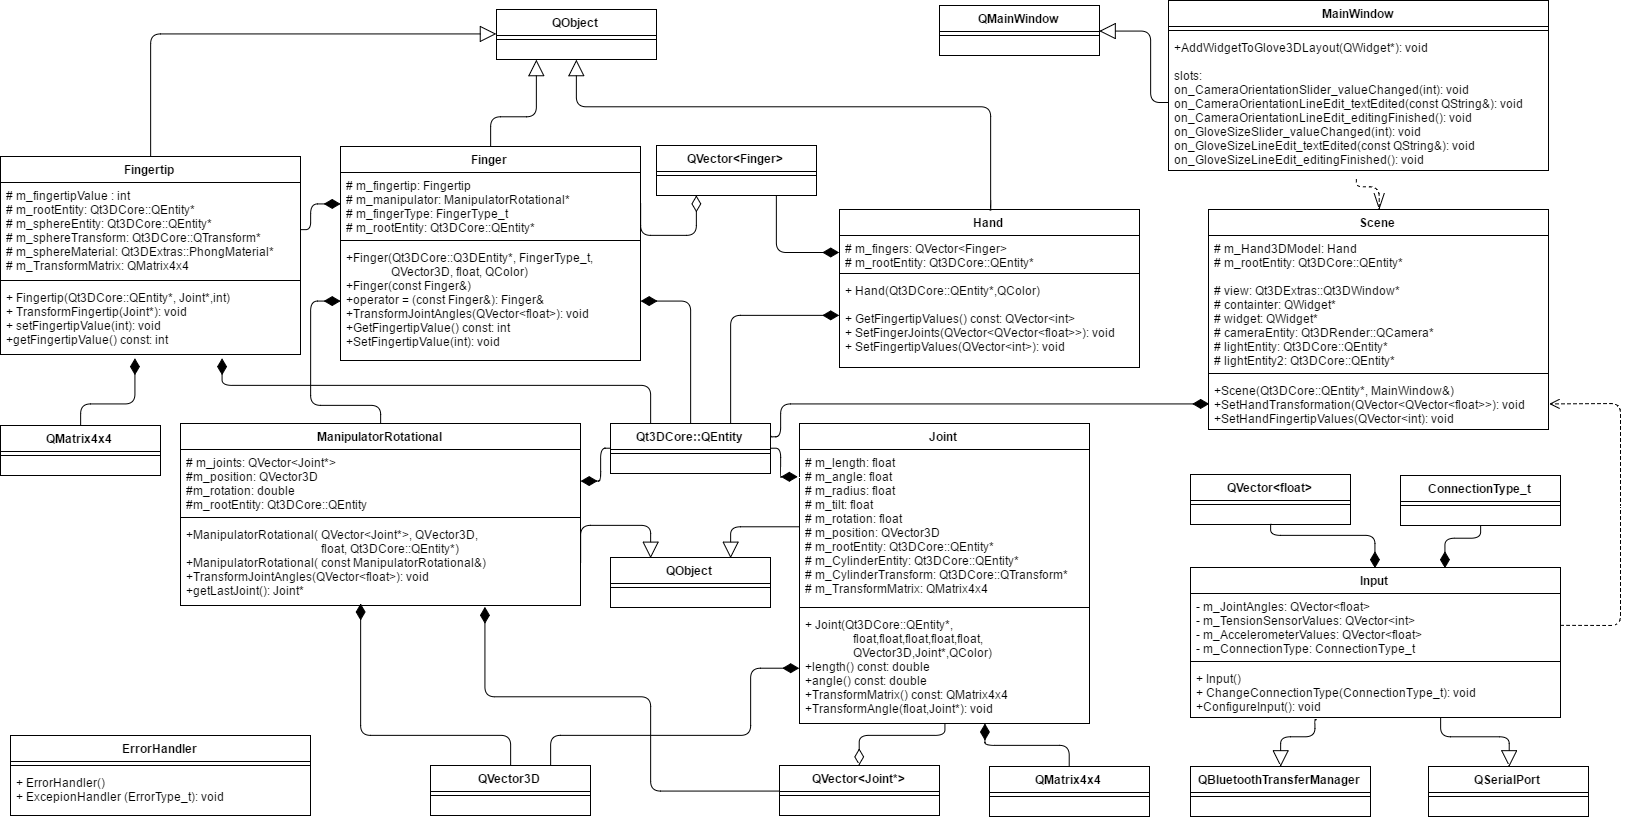
\includegraphics[angle=90,height=0.8\textheight]{./ClassDiagram.png}
\caption{Diagram klas części aplikacji odpowiedzialnej za przetwarzanie danych\label{fig:classdiagram}}
\end{figure}
\newpage
\subsection{Diagram czynności}
\begin{figure}[!htb]
\centering
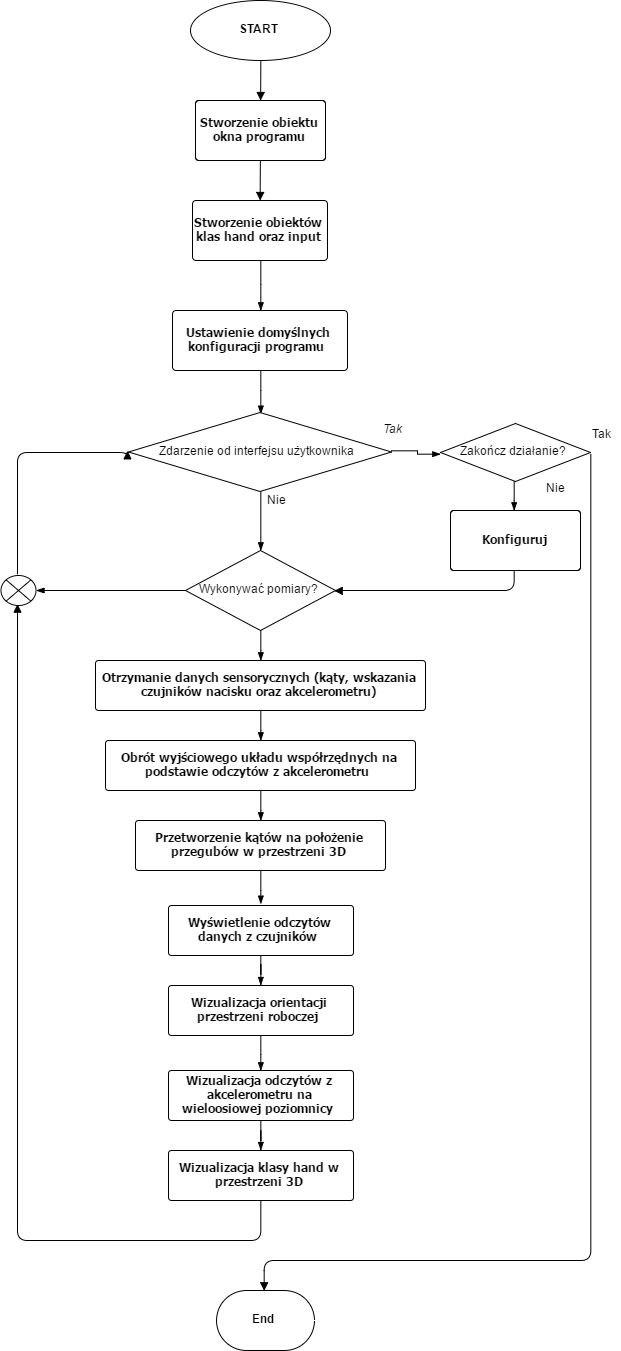
\includegraphics[height=0.8\textheight]{./Diagram_przeplywu_sterowania.png}
\caption{Diagram czynności}
\end{figure}

\newpage
\subsection{Wyniki eksperymentów}
Przeprowadzono eksperymenty z użyciem dłoni sensorycznej i aplikacji napisanej w ramach tego projektu, polegające na wizualizacji kilku prostych gestów i określeniu sposobu ich identyfikacji. Wyniki eksperymentów zostały przedstawione na rysunkach (\ref{fig:Fist}, \ref{fig:Palm}, \ref{fig:OK}, \ref{fig:Peace}, \ref{fig:Point}).\\
\begin{figure}[!htb]
\centering
    \subfloat
    {
      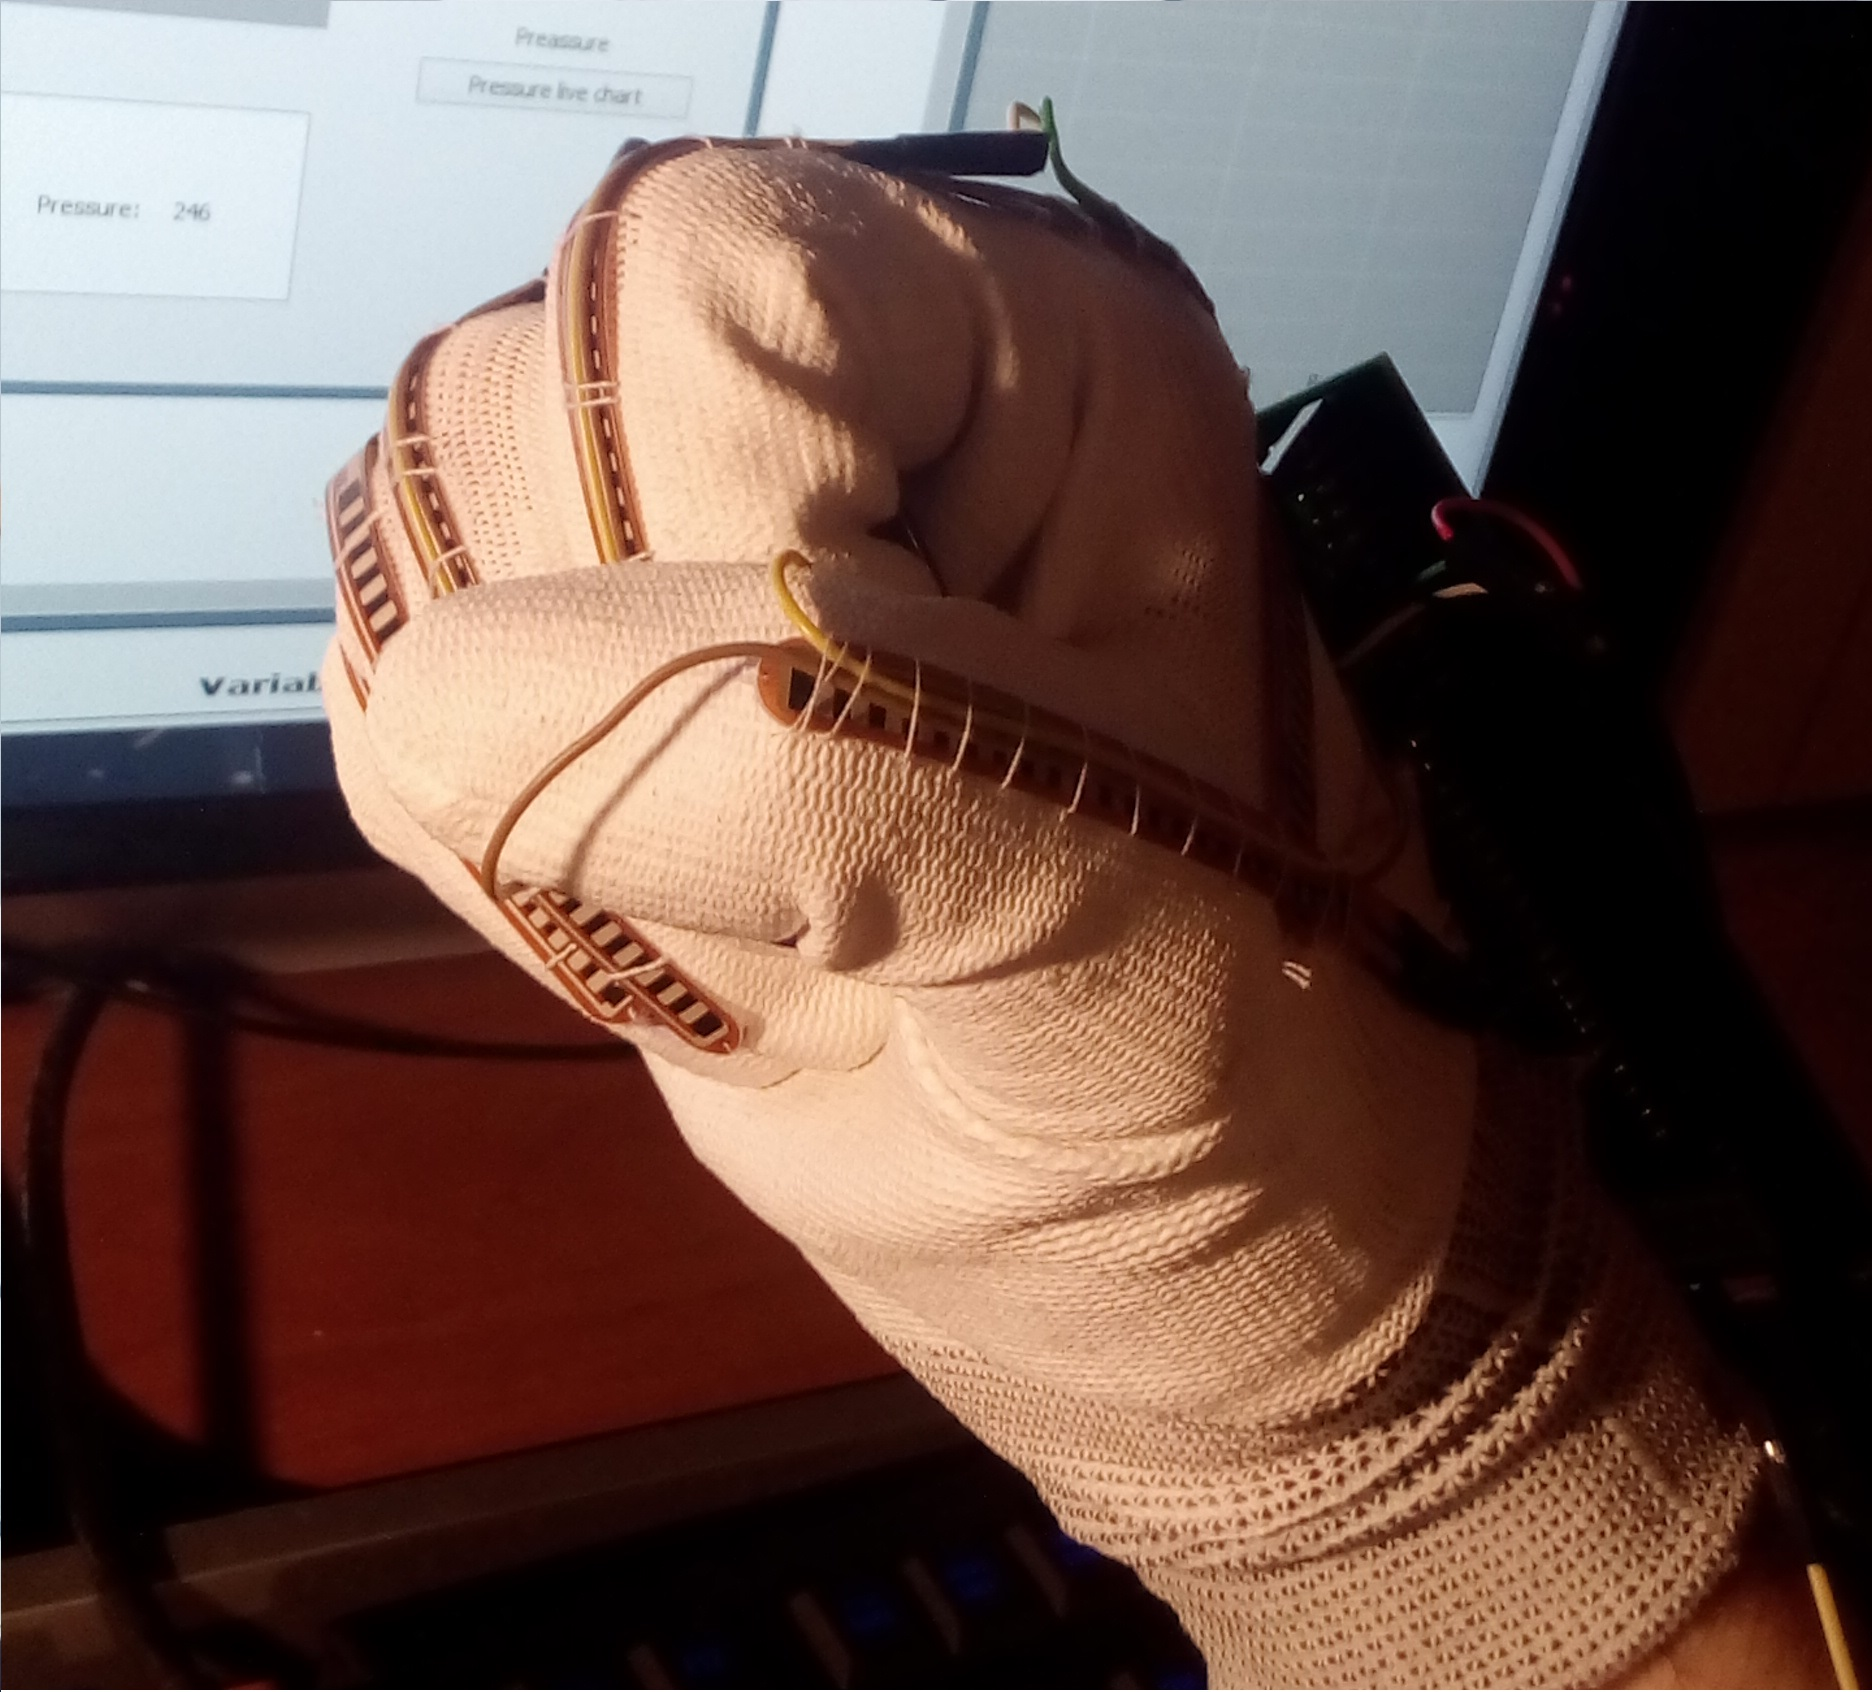
\includegraphics[width=0.48\textwidth]{./Fist.jpg}
    }
    \subfloat
    {
      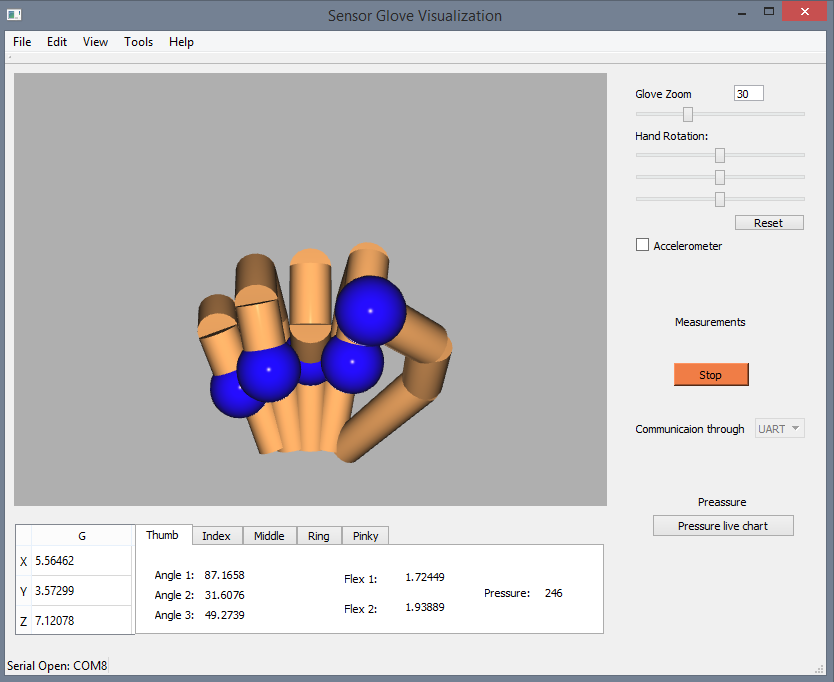
\includegraphics[width=0.48\textwidth]{./FistQt.png}
    }
    \caption{Gest -- zaciśnięta pięść \label{fig:Fist}}
\end{figure}
\begin{figure}[!htb]
\centering
    \subfloat
    {
      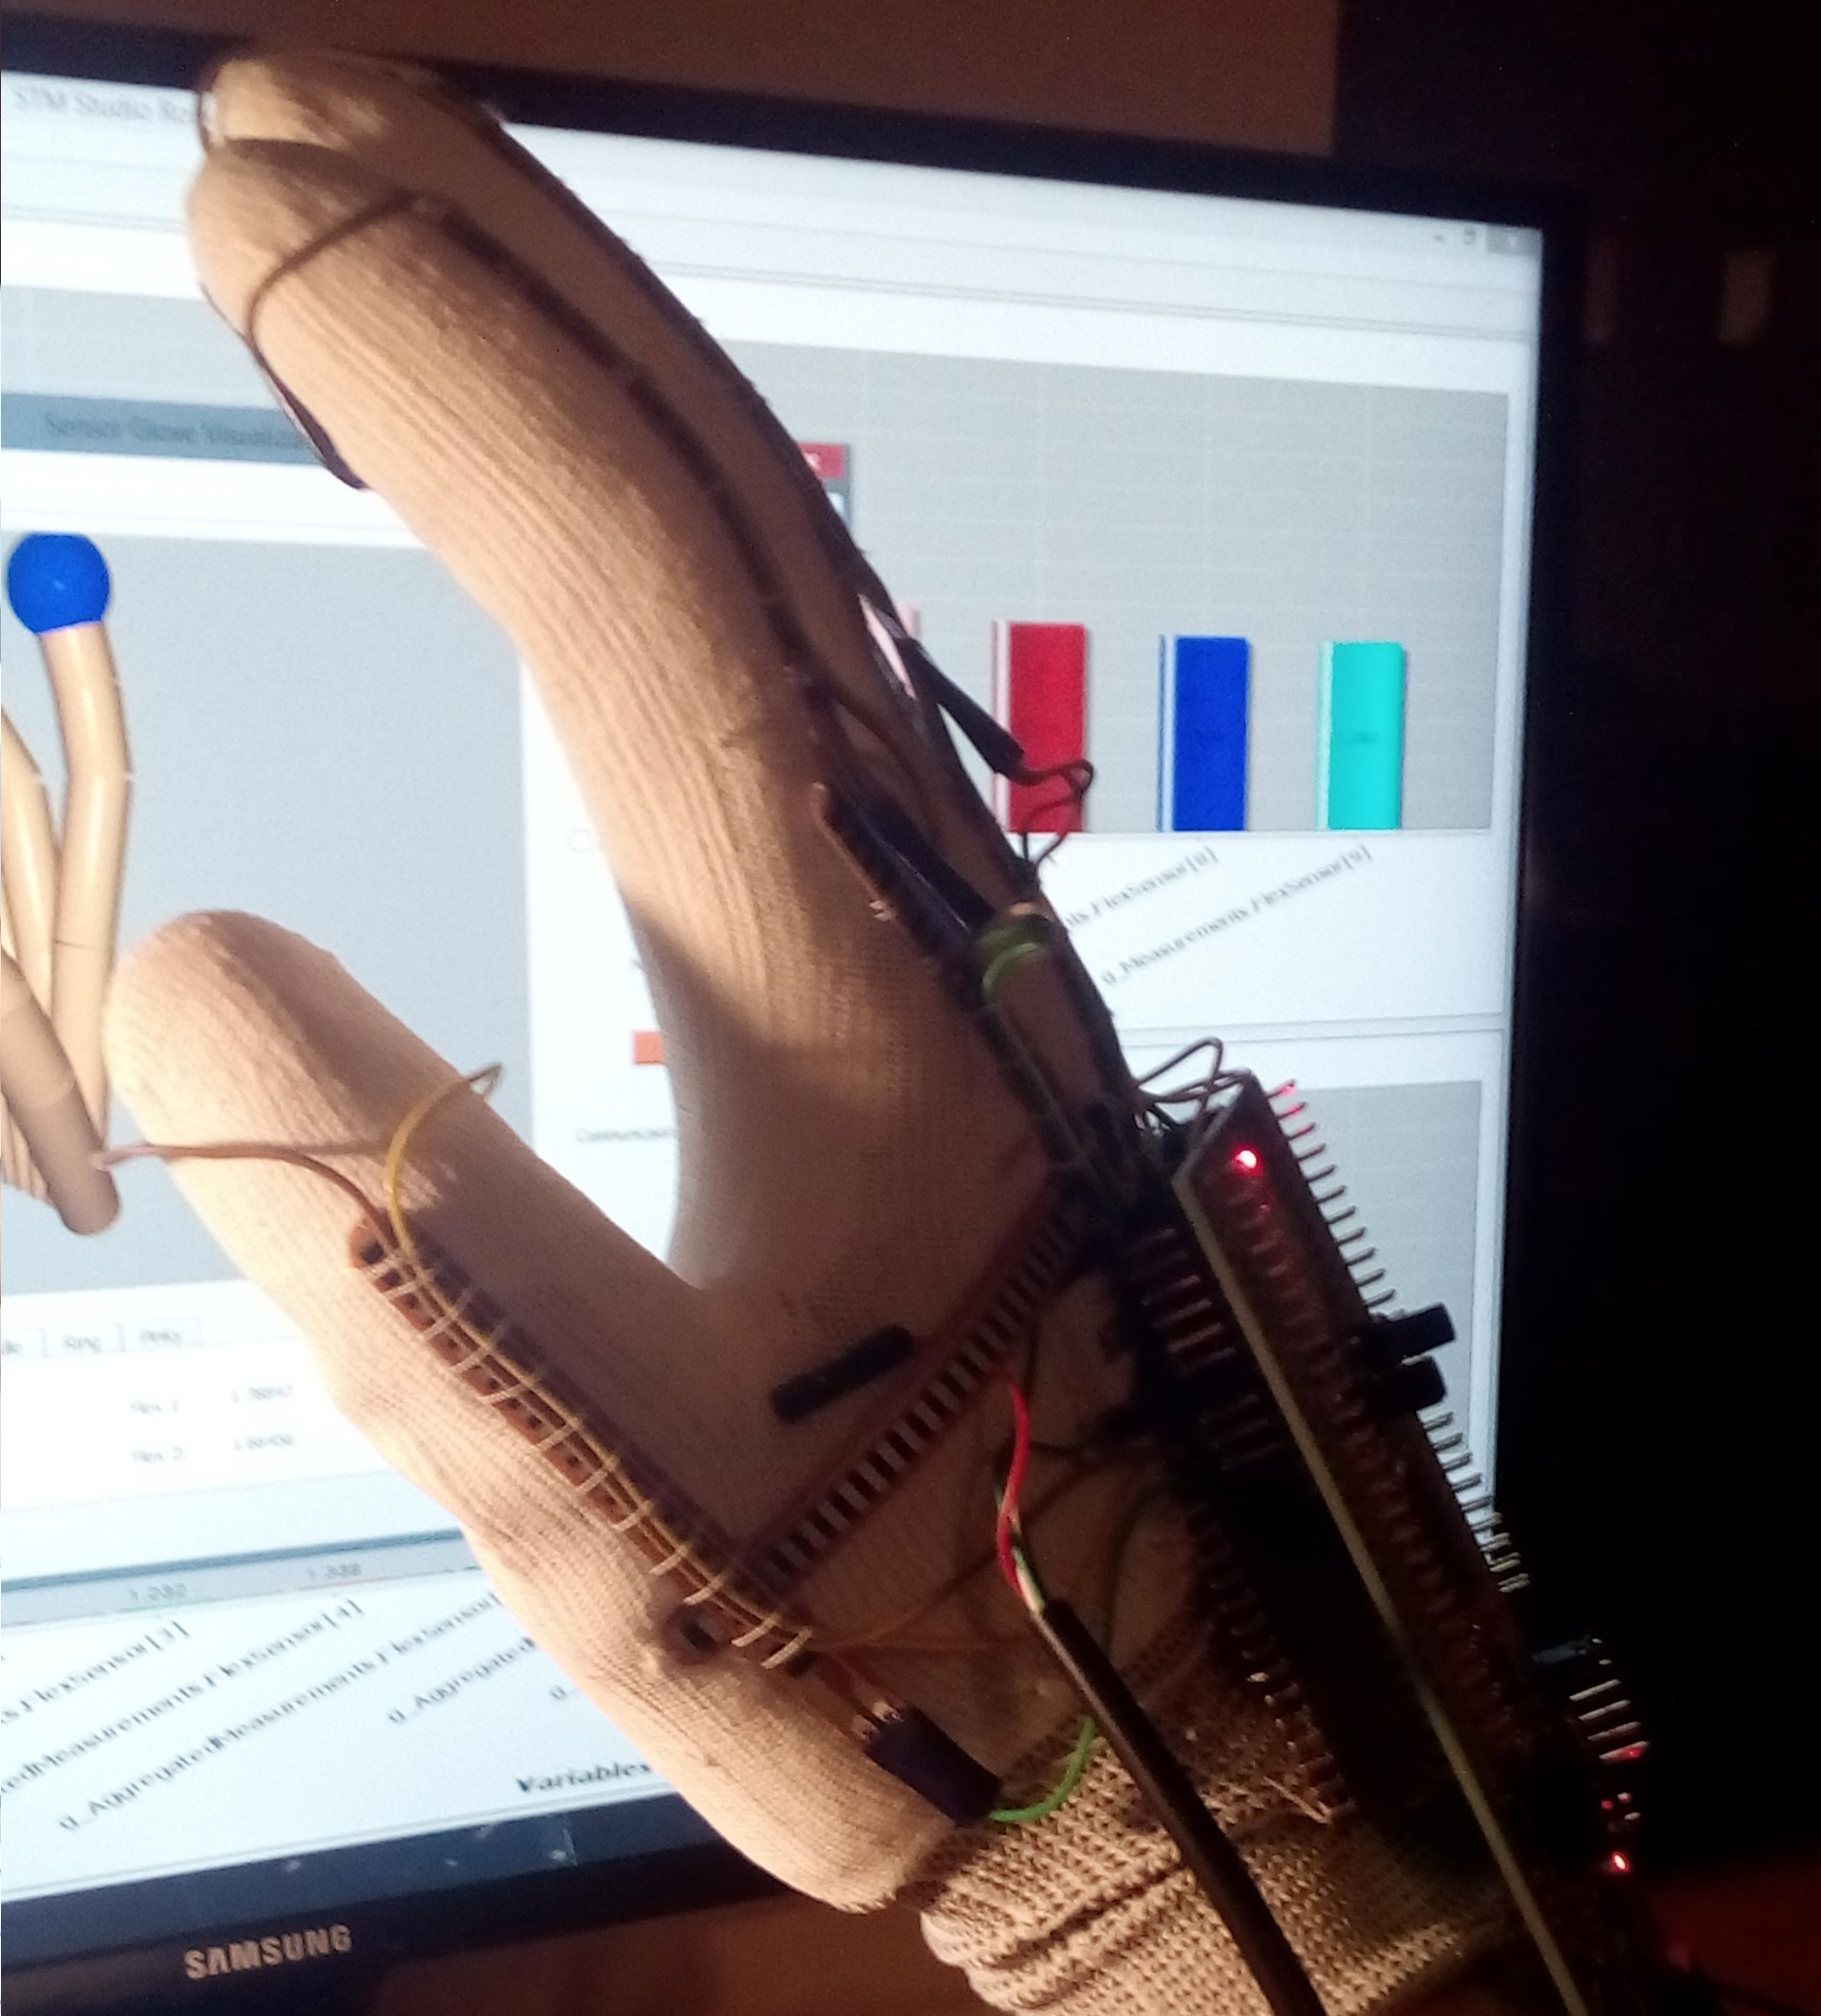
\includegraphics[width=0.48\textwidth]{./Palm.jpg}
    }
    \subfloat
    {
      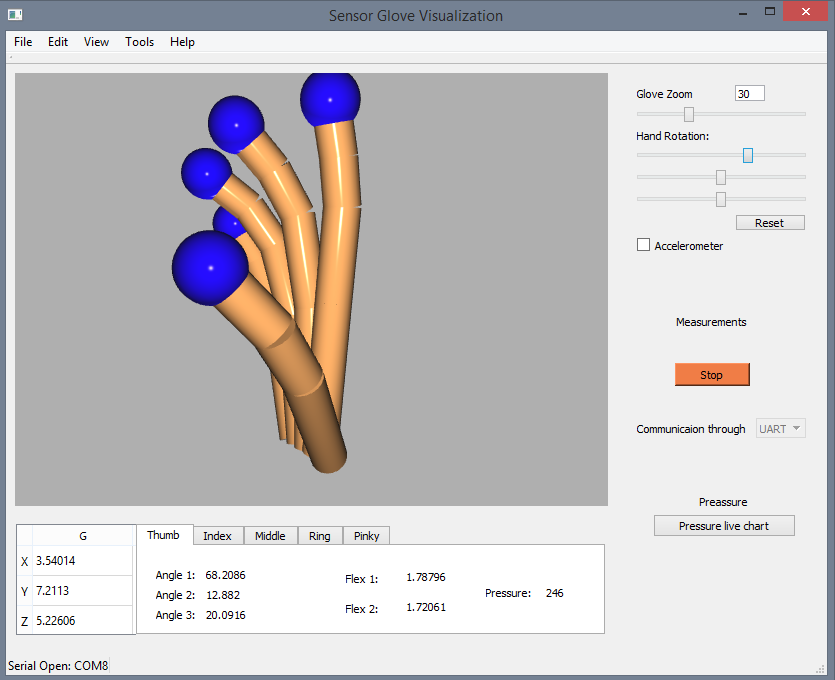
\includegraphics[width=0.48\textwidth]{./PalmQt.png}
    }
    \caption{Gest -- otwarta dłoń \label{fig:Palm}}
\end{figure}
\begin{figure}[!htb]
\centering
    \subfloat
    {
      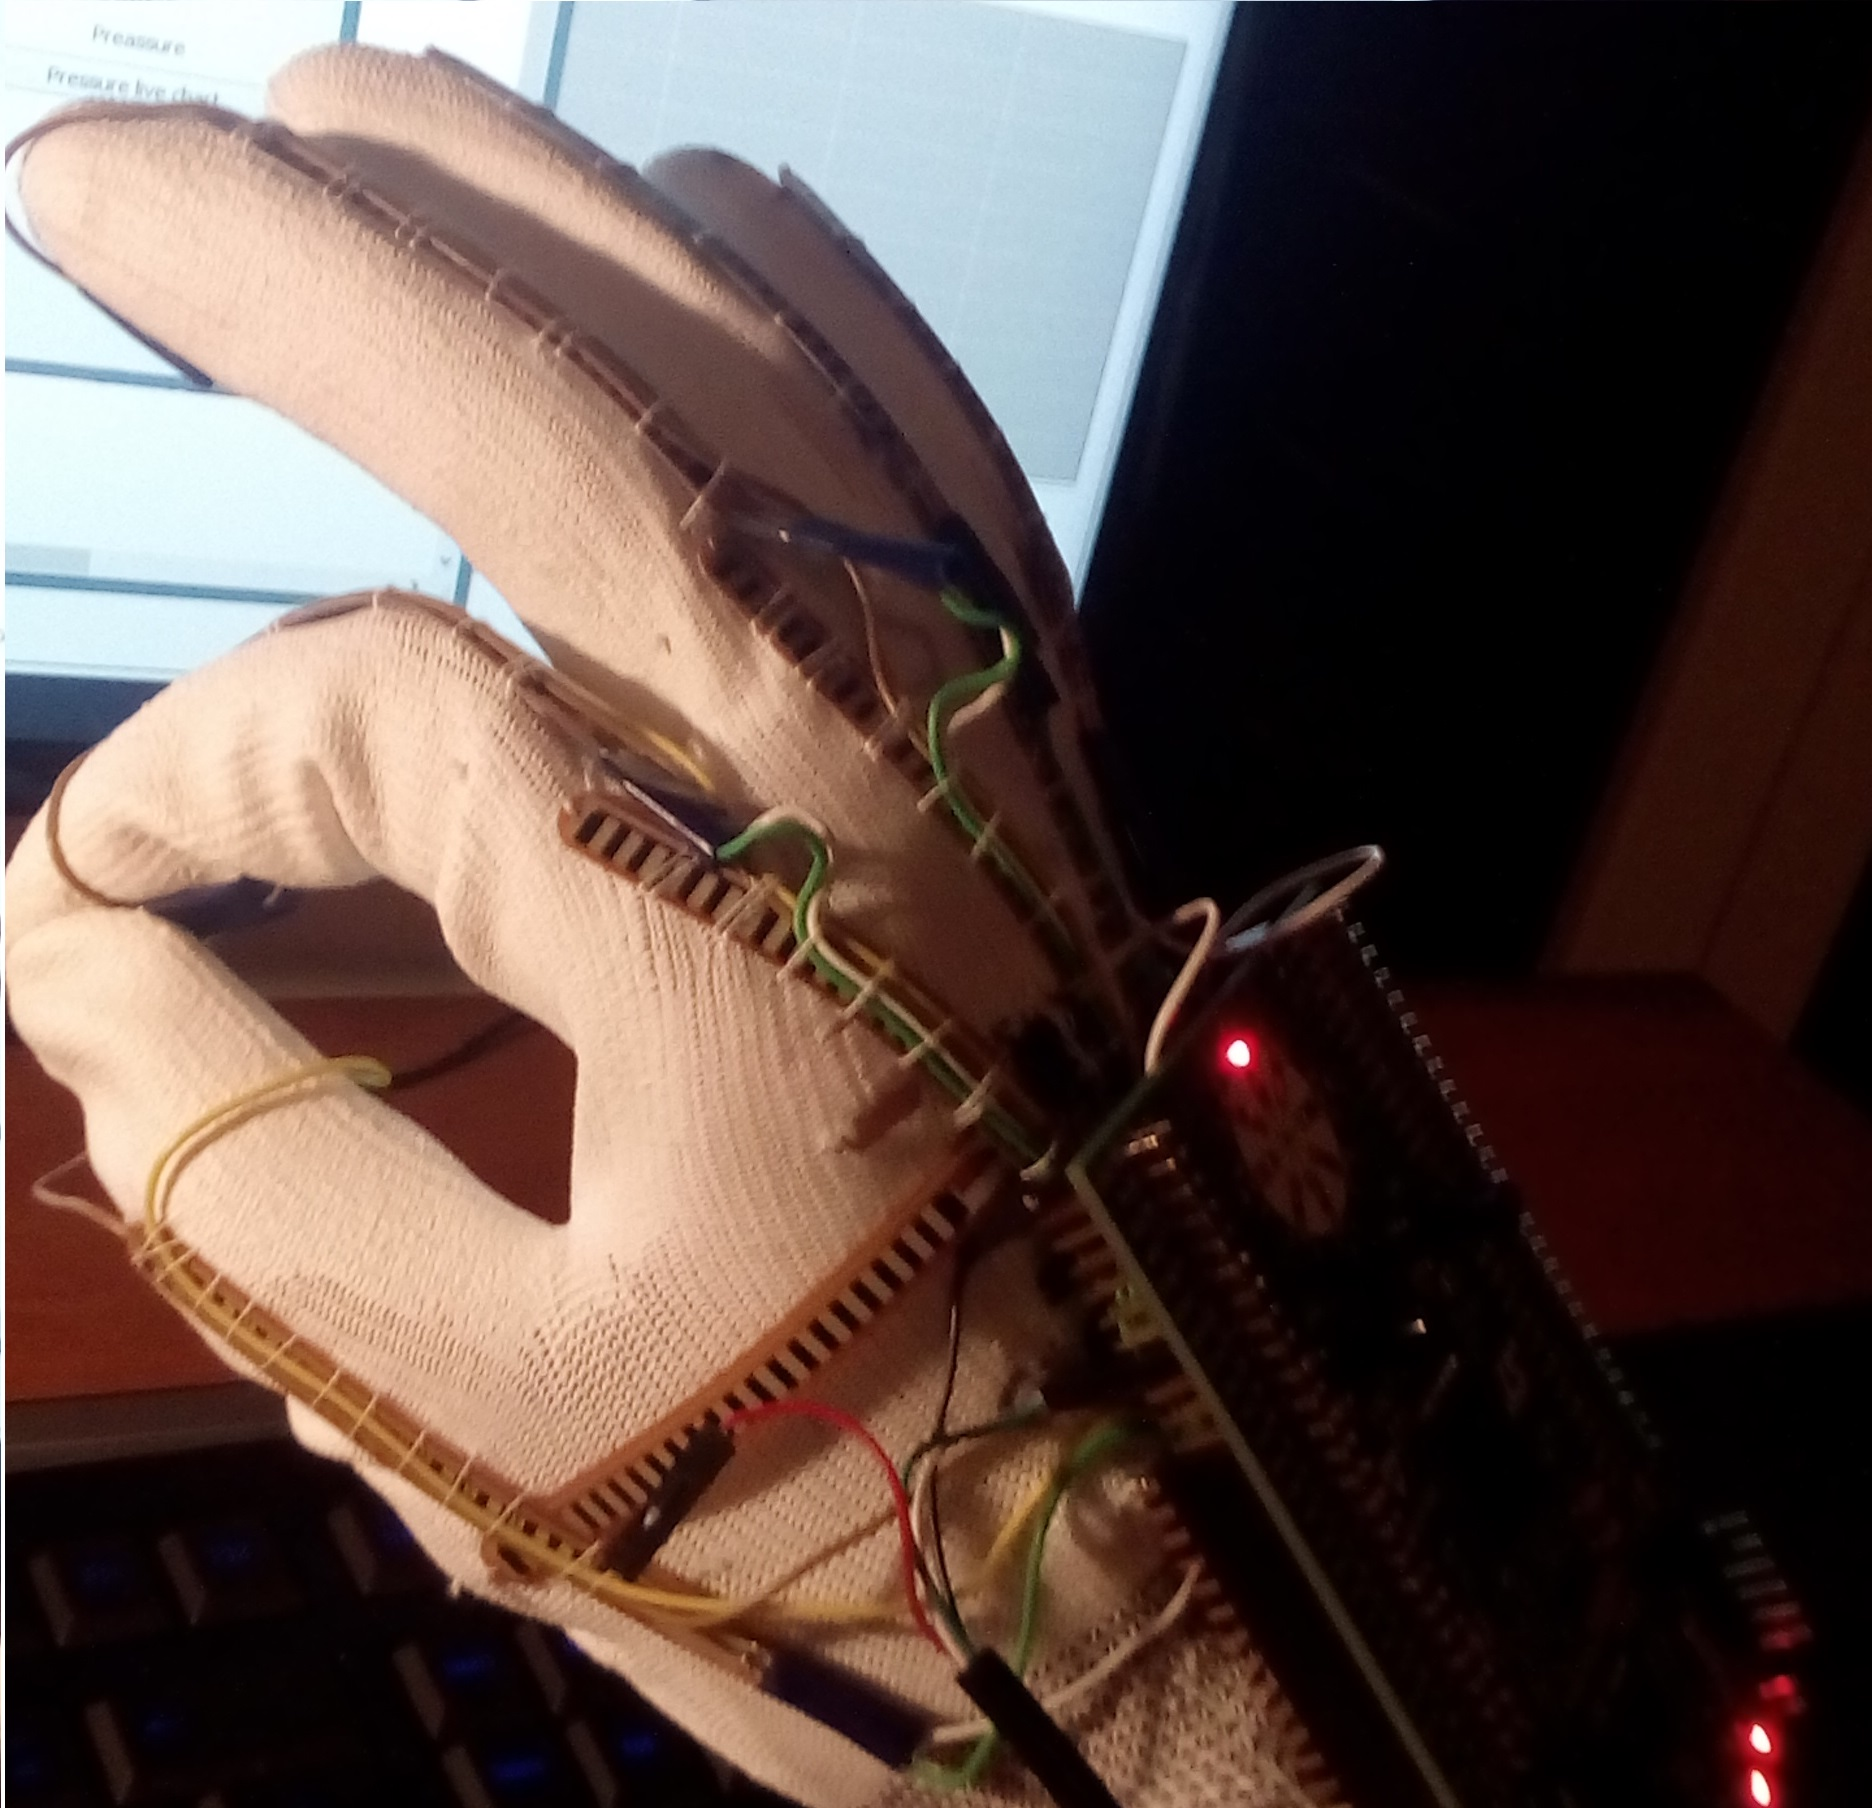
\includegraphics[width=0.48\textwidth]{./OK.jpg}
    }
    \subfloat
    {
      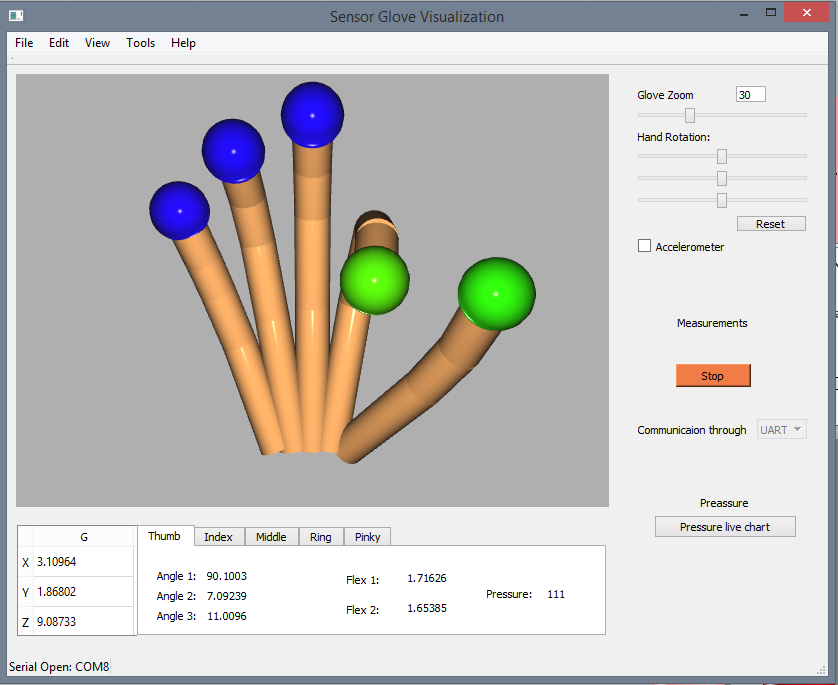
\includegraphics[width=0.48\textwidth]{./OKQt.png}
    }
    \caption{Gest -- OK \label{fig:OK}}
\end{figure}
\begin{figure}[!htb]
\centering
    \subfloat
    {
      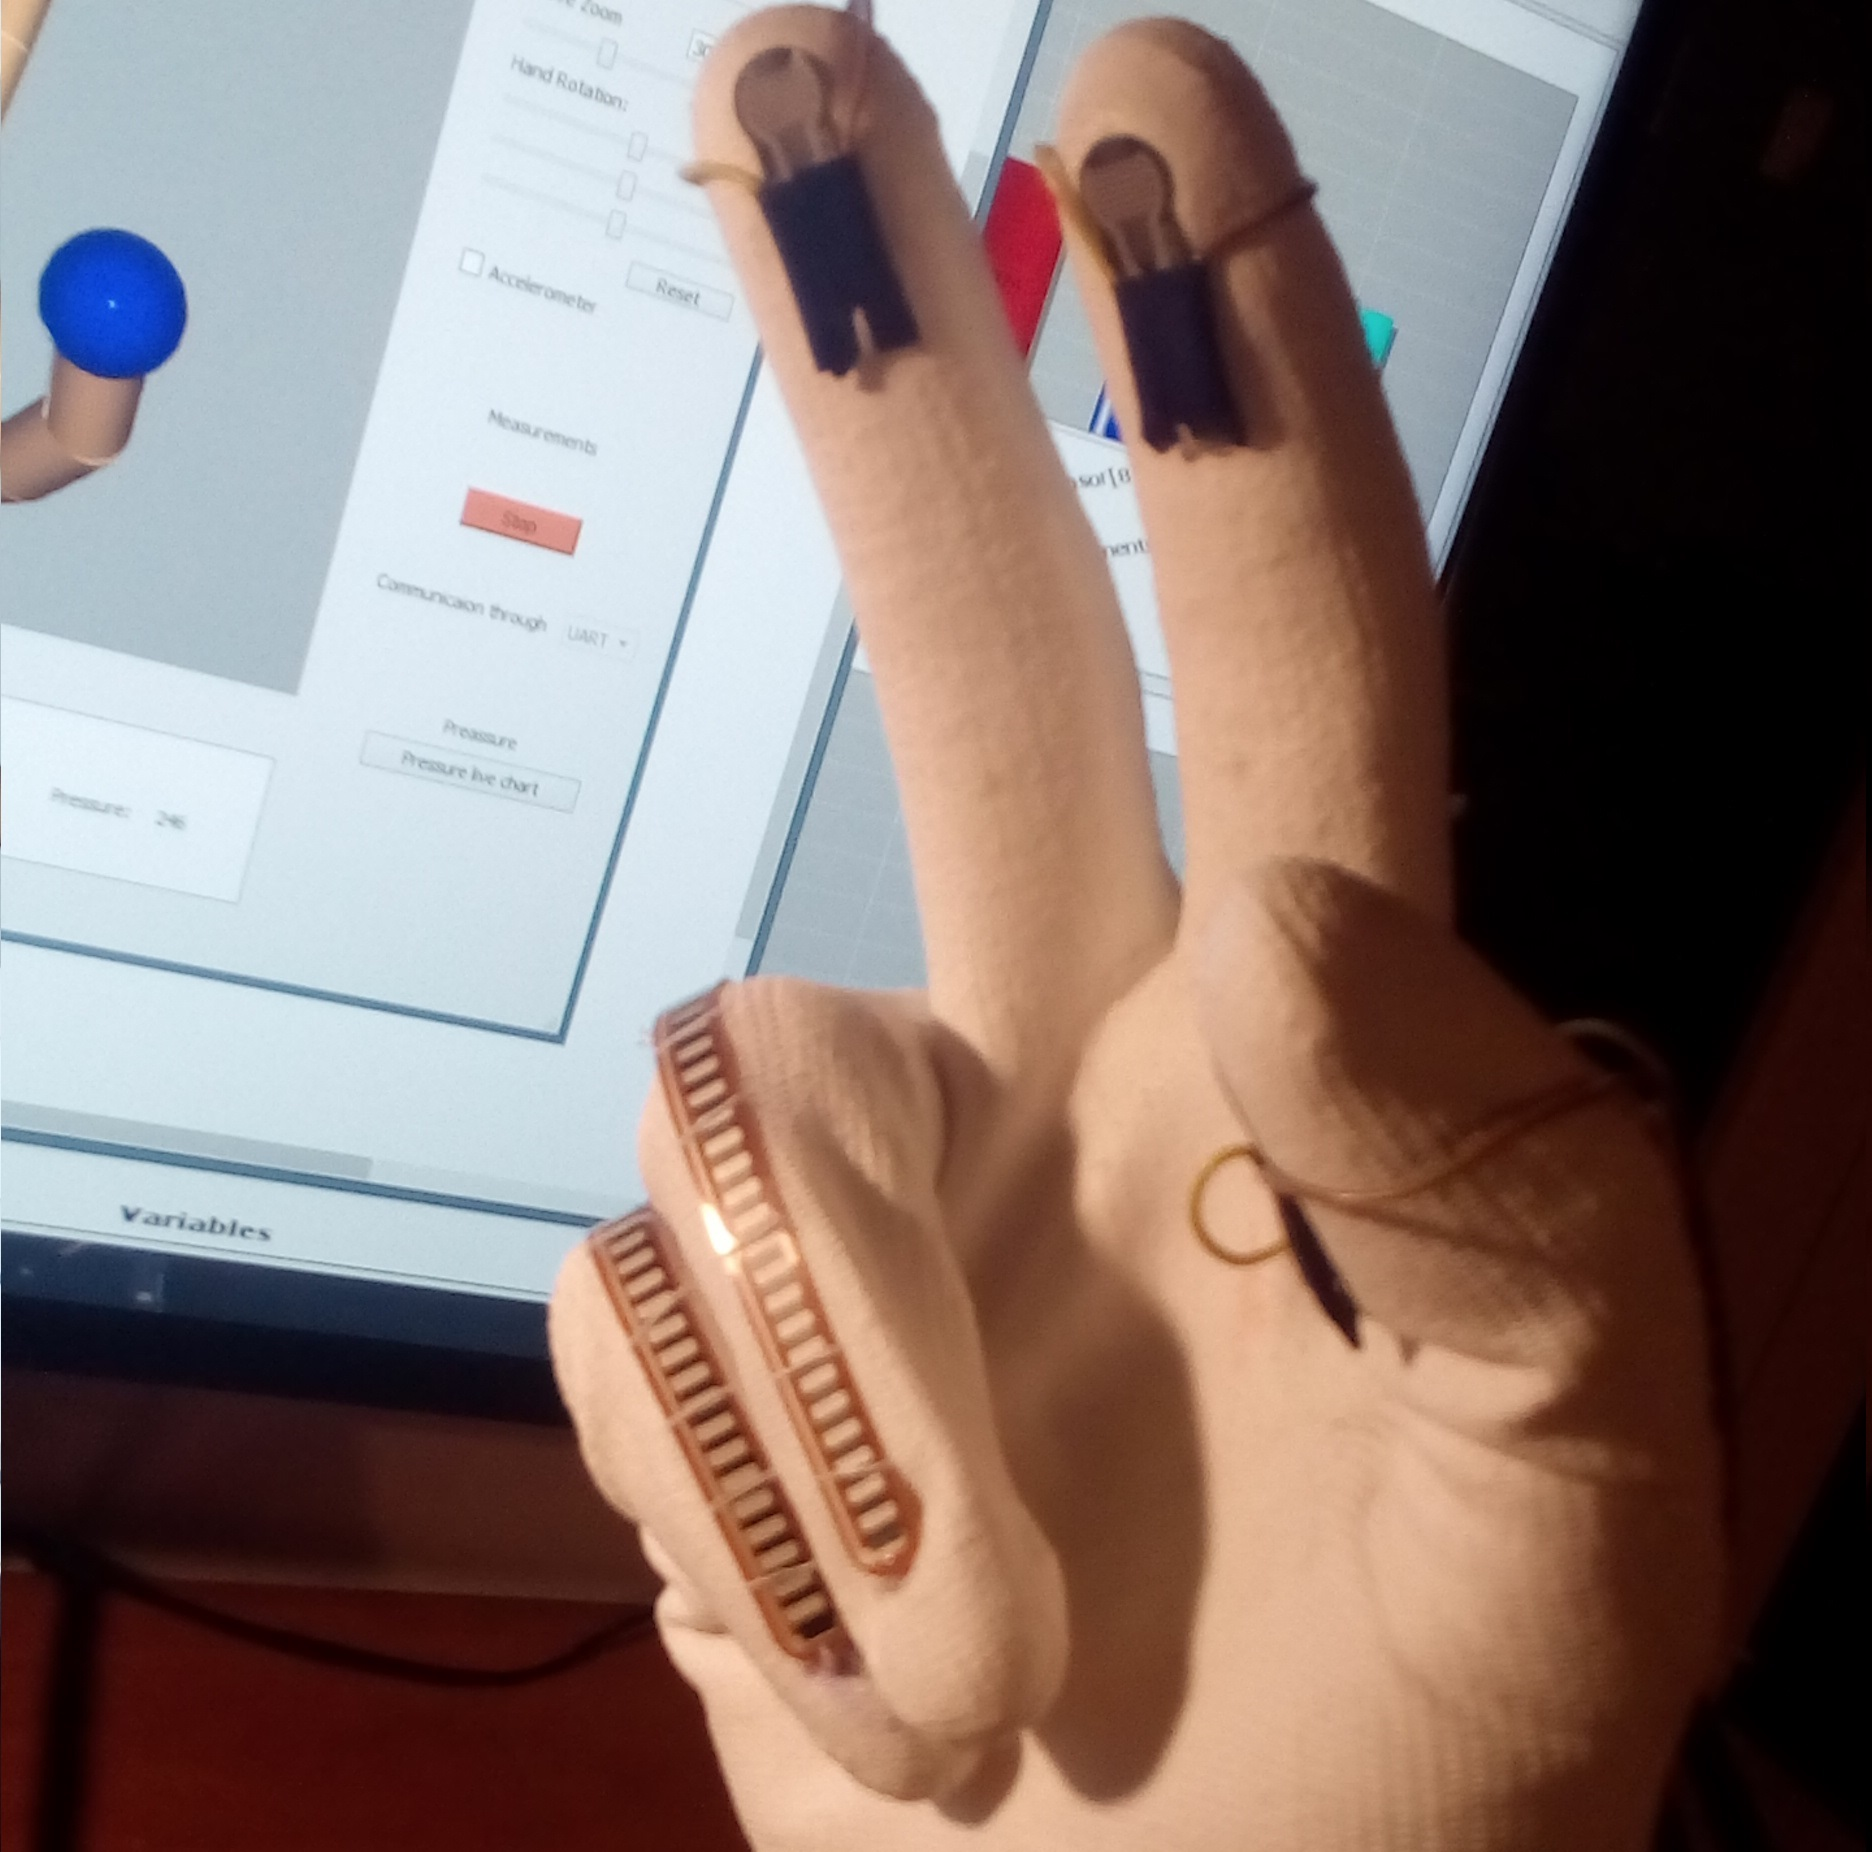
\includegraphics[width=0.48\textwidth]{./Peace.jpg}
    }
    \subfloat
    {
      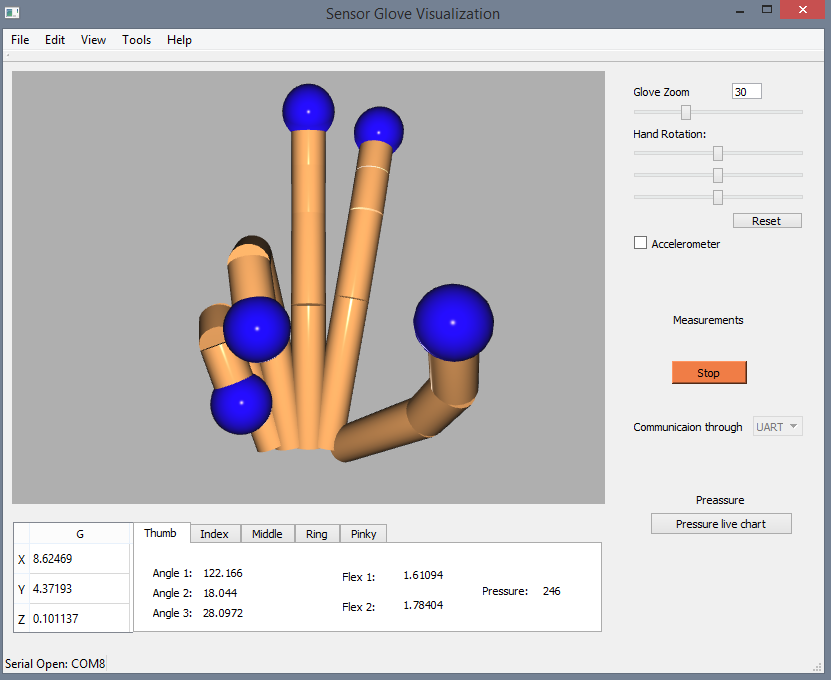
\includegraphics[width=0.48\textwidth]{./PeaceQt.png}
    }
    \caption{Gest -- pacyfka\label{fig:Peace}}
\end{figure}
\begin{figure}[!htb]
\centering
    \subfloat
    {
      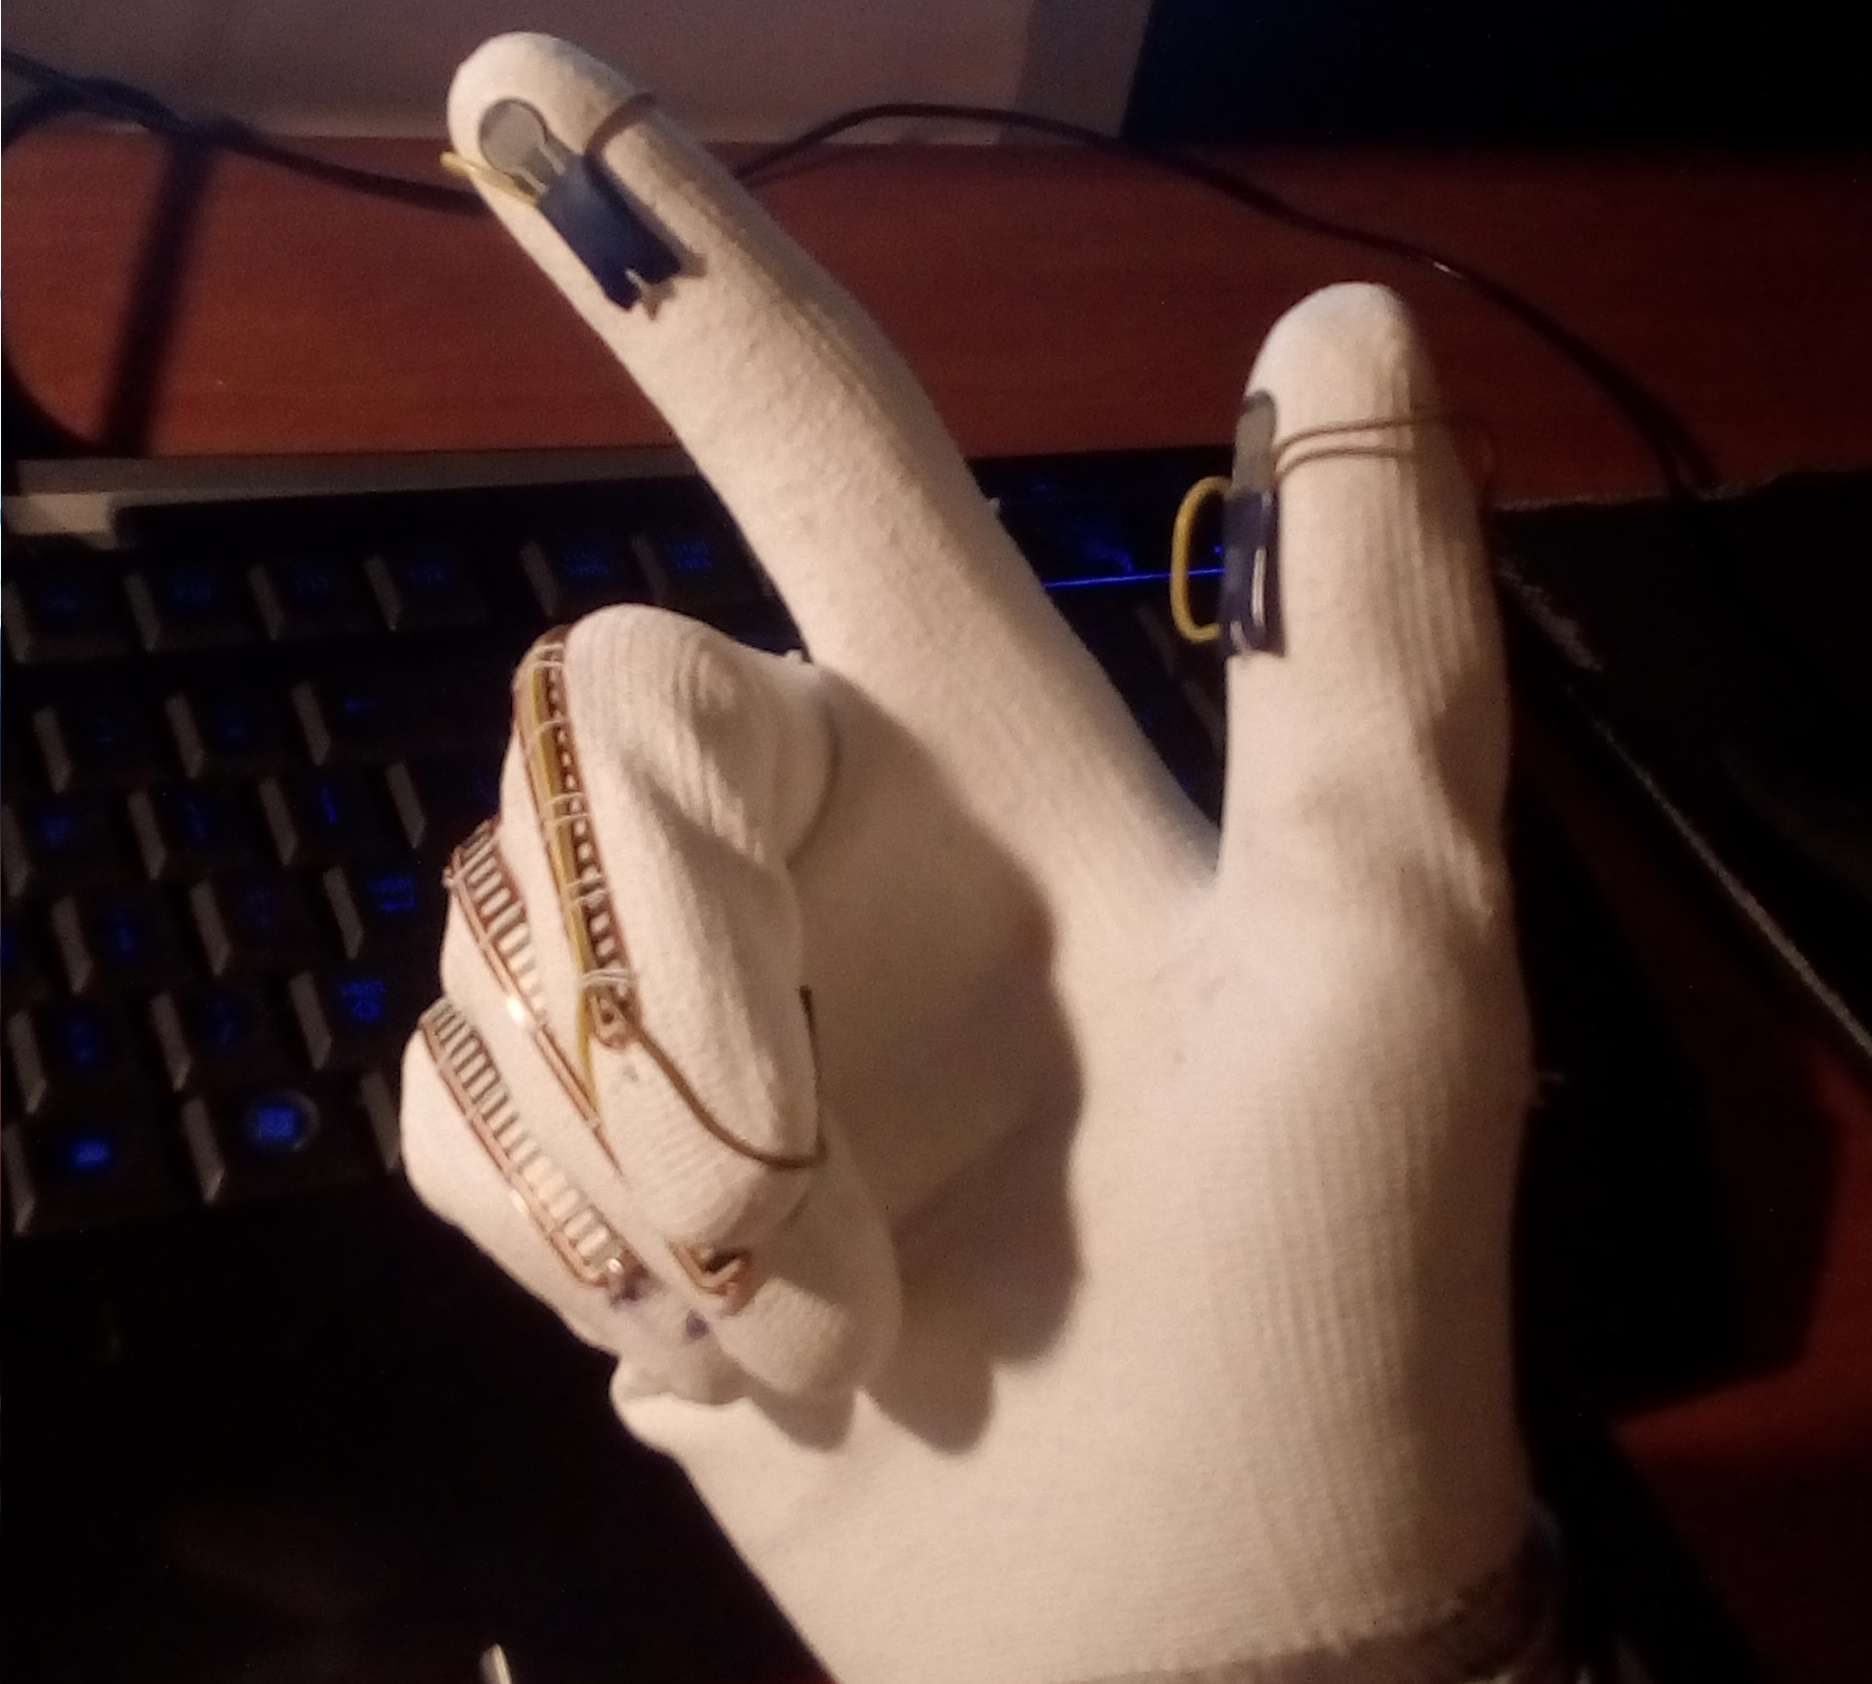
\includegraphics[width=0.48\textwidth]{./Point.jpg}
    }
    \subfloat
    {
      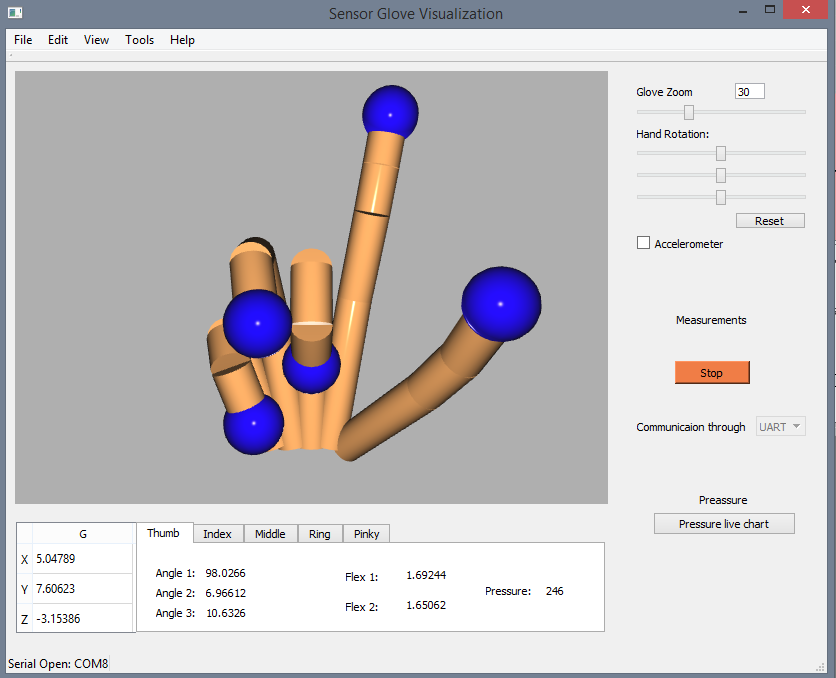
\includegraphics[width=0.48\textwidth]{./PointQt.png}
    }
    \caption{Gest -- wskazywanie palcem \label{fig:Point}}
\end{figure}
Wykrywanie tego typu gestów sprowadza się do ustawienia odpowiednich progów na niektórych czujnikach ugięcia i nacisku, po których przekroczeniu sygnalizuje się wykrycie gestu.\\
Takie gesty mogą posłużyć sterowaniu robotem lub systemem automatyki (np. budynkowej). Przyporządkowanie gestu do wykonywanej czynności daje możliwość kontroli systemu.

\newpage
\section{Specyfikacja urządzenia}

\subsection{Opis ogólny}
\begin{itemize}
\item Na opuszkach palców zamontowane zostaną czujniki siły nacisku FSR--400. Spadek rezystancji przy przyłożonej sile pozwala zmierzyć siłę nacisku.
\item Do wykrycia zgięcia stawów międzypaliczkowych bliższych oraz stawu międzypaliczkowego kciuka zastosowane zostaną czujniki ugięcia -- flexsensory firmy Sparkfun. Zgięcie tych sensorów powoduje wzrost rezystancji.
\item Akcelerometr LSM303DLHC, znajdujący się na płytce Discovery zostanie użyty do określenia orientacji rękawicy względem wektora grawitacji.
\item Powyższe elementy nie zapewniają precyzyjnych pomiarów, ale zostały wybrane ze względu na cenę i charakter projektu, w którym zostaną zastosowane.
\item Jako urządzenie nadawcze Bluetooth posłuży moduł HC--06 z interfejsem UART podłączony do płytki Discovery.
\end{itemize}
Rękawica sensoryczna tworzona w ramach projektu Roboty Mobilne została zbudowana.

\subsection{Funkcjonalności urządzenia}
\begin{itemize}
\item Pobieranie danych o nacisku opuszków palców na powierzchnię.
\item Pobieranie danych o zgięciu palców dłoni.
\item Pobieranie danych o orientacji względem wektora grawitacji.
\item Agregacja danych do odpowiednich jednostek.
\item Aproksymacja danych w celu określenia kątów ugięcia oraz kątów rotacji (RPY).
\item Wysyłanie danych przez USB, UART, Bluetooth.
\item Wizualizacja nacisku opuszków palców na powierzchnię za pomocą LEDów RGB. (niezrealizowane)
\end{itemize}

\newpage
\subsection{Schematy układu elektronicznego}
W ramach projektów Wizualizacja Danych Sensorycznych oraz Roboty Mobilne, nie jest przygotowywany własny układ elektroniczny. Połączenia za pomocą przewodów z płytką sterującą oddaje schemat ideowy.
Ideowy schemat połączeń urządzenia pomiarowego, współpracującego z aplikacją został przedstawiony na rysunku \ref{fig:ideascheme}.
\begin{figure}[!htb]
\centering
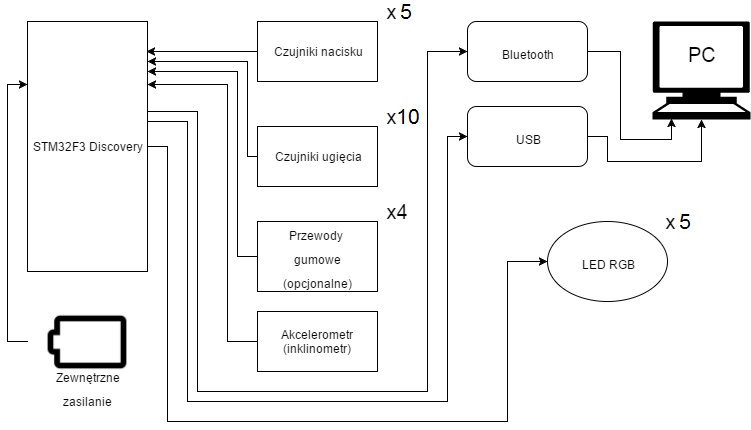
\includegraphics[width=0.9\textwidth]{./SchematIdeowy.png}
\caption{Ideowy schemat połączeń rękawicy sensorycznej\label{fig:ideascheme}}
\end{figure}
Schematy elektroniki głównej płytki z mikrokontrolerem urządzenia pomiarowego można znaleźć na stronie producenta. Rysunek ułożenia elementów na płytce został ukazany na rysunku \ref{fig:layout}.
\begin{figure}[!htb]
\centering
\subfloat
{
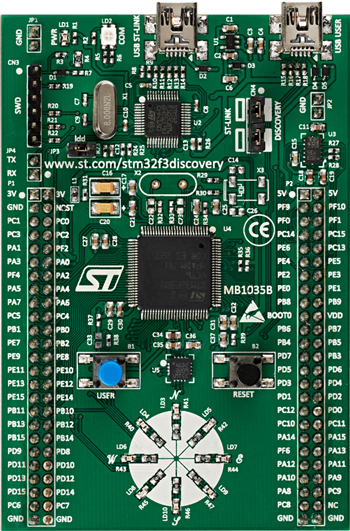
\includegraphics[height=0.6\textwidth]{32f3discovery.jpg}
}
\subfloat
{
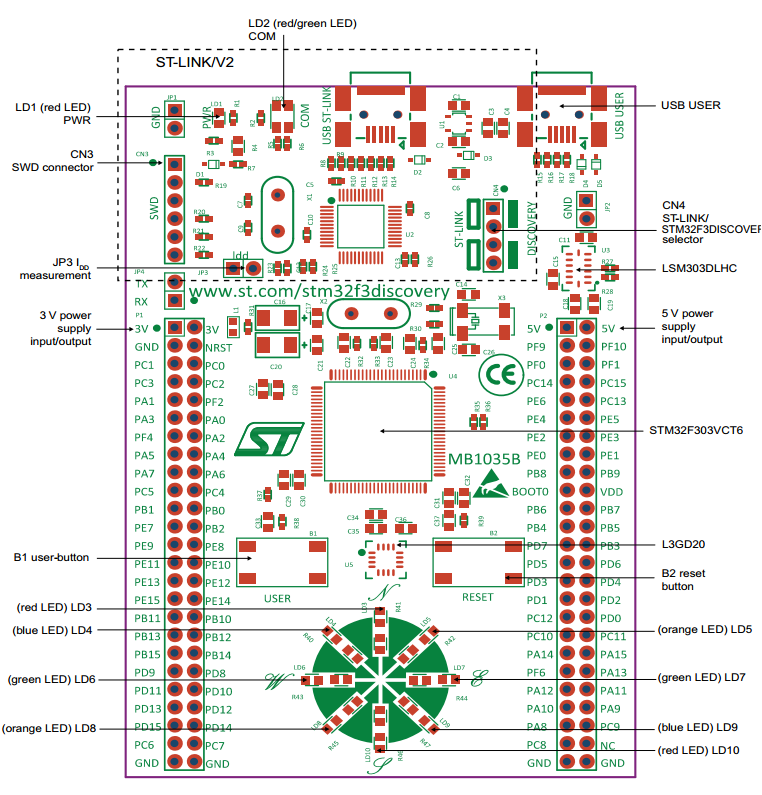
\includegraphics[height=0.6\textwidth]{stm32f3layout.png}
}
\caption{Fizyczne ułożenie elementów na płytce PCB\label{fig:layout}}
\end{figure}

\newpage
\subsection{Parametry układu pomiarowego}
\subsubsection{Konfiguracja przetwornika pomiarowego}
\begin{itemize}
\item Rozdzielczość przetwornika: 12 bitów
\item Zakres pomiarowy: (0 -- 4095: int), (0 -- 3,3 V)
\item Pomiar ciągły z wykorzystaniem DMA
\item Czas próbkowania: 181,5 Cykli
\item Częstotliwość zegara: 32 MHz
\end{itemize}

\subsubsection{Dane czujnika ugięcia}
\begin{itemize}
\item Długość powierzchni czynnej: 55,37 mm
\item Zakres rezystancji: 25 -- 125 k$\Omega$
\item Rezystor pomiarowy do dzielnika: 62 k$\Omega$
\end{itemize}
\subsubsection{Dane czujnika nacisku}
\begin{itemize}
\item Średnica powierzchni czynnej: 5 mm
\item Zakres pomiarowy nacisku: 0,2 -- 20 N
\item Zakres rezystancji: 150 -- 10 M$\Omega$
\item Rezystor pomiarowy do dzielnika: 3 k$\Omega$
\end{itemize}
\subsubsection{Dane z akcelerometru}
\begin{itemize}
\item Protokół komunikacyjny: $I^2C$
\item Ilość osi: 3
\item Maksymalne przeciążenie: $\pm$16g
\item Dokładność pomiaru: 16 bitów 
\end{itemize}

\subsection{Opis protokołu komunikacji}
Wykorzystano trzy sposoby komunikacji z urządzeniem pomiarowym. Możliwość przełączania między urządzeniami została przewidziana w aplikacji. Dane odbierane z rękawicy zostaną wstępnie przetworzone przez urządzenie pomiarowe.\\
\subsection{Ramka danych}
\begin{itemize}
\item Typ danych: float
\item Sposób odbierania danych: COM Port (QSerialPort)
\item Sposób kodowania wiadomości: ANSI
\item Suma kontrolna: brak
\item Struktura wiadomości: 1 linia danych
\begin{itemize}
\item Znak początku 'S'
\item 15x float -- kąty obrotu przegubów palców $(\pm 180,0 ^\circ$)
\item 5x int -- dane z czujników nacisku (0 -- 255)
\item 3x float -- kąty obrotu parametryzacji Roll Pitch Yaw $(\pm 180,0^\circ$)
\item 3x float -- przyśpieszenie w trzech osiach XYZ $(\pm 18 \frac{m}{s^2})$
\item 10x float -- odczyty czujników ugięcia (0,0 -- 3,3 V)
\item Znak końca 'R'
\item Linia zakończona znakami \textbackslash r \textbackslash n
\end{itemize}
\item Zrezygnowano ze szczegółowego opisu niskopoziomowego ramki danych, gdyż jest on obsługiwany przez dostępne biblioteki
\end{itemize}
\subsubsection{Bluetooth}
\begin{itemize}
\item Nazwa modułu komunikacyjnego: HC -- 06
\item Interfejs komunikacyjny ze strony urządzenia: UART
\item Interfejs komunikacyjny ze strony aplikacji: Serial COM Port / moduł QtBluetooth
\item Baud Rate: 9600 b/s
\item Długość słowa: 8 bit
\item Parzystość: brak
\item Bity stopu: 1
\item Nadpróbkowanie: 16 próbek
\item Wykorzystanie przerwań i/lub DMA
\end{itemize}
\subsubsection{USB -- Serial Port}
\begin{itemize}
\item Nazwa modułu komunikacyjnego: Wbudowany
\item Interfejs komunikacyjny ze strony urządzenia: USB Device (FS)
\item Interfejs komunikacyjny ze strony aplikacji: Serial COM Port
\item Szybkość: 12 Mb/s
\item Maksymalna wielkość pakietu: 64 B
\end{itemize}

\newpage
%Rozpisać na kolejne tygodnie
\section{Harmonogram}
\begin{itemize}
\item (31.03.2017) \textbf{(Wykonane)} Uruchomienie i przetestowanie pętli USB$\rightarrow $UART$\rightarrow $USB w celu symulacji danych sensorycznych. 
\item (14.04.2017) \textbf{(Wykonane)} Stworzenie struktur danych wykorzystywanych w aplikacji (przeguby, manipulatory, scena).
\item (14.04.2017) \textbf{(Wykonane)} Stworzenie projektu okna programu.
% Wstępne rezultaty
\item (05.05.2017) \textbf{(Wykonane)} Stworzenie uproszczonego modelu kośćca dłoni.
\item (14.05.2017) \textbf{(Wykonane)} Stworzenie elementów wizualizacji nacisku.
\item (18.05.2017) \textbf{(Wykonane)} Zmiana koloru i/lub wielkości sfer na podstawie odczytów z czujników nacisku.
%Rezultaty prawie końcowe
\item (26.05.2017) \textbf{(Zrezygnowano)} Komunikacja przez Bluetooth.
\item (26.05.2017) \textbf{(Wykonane)} Komunikacja przez USB.
\item (01.06.2017) \textbf{(Wykonane)} Stworzenie okna programu.
\item (01.06.2017) \textbf{(Wykonane)} Wczytywanie i dekodowanie danych z rękawicy sensorycznej.
\item (05.06.2017) \textbf{(Wykonane)} Poruszanie przegubami na podstawie odczytów z tensorów.
\item (05.06.2017) \textbf{(Wykonane)} Obrót modelu na podstawie akcelerometru.
\item (11.06.2017) \textbf{(Wykonane)} Testy aplikacji.
\item (15.06.2017) \textbf{(Wykonane)} Naprawianie błędów.
\item (15.06.2017) \textbf{(Częściowo wykonane)} Poprawianie funkcjonalności i optymalizacja kodu.
%Rezultaty końcowe
\end{itemize}

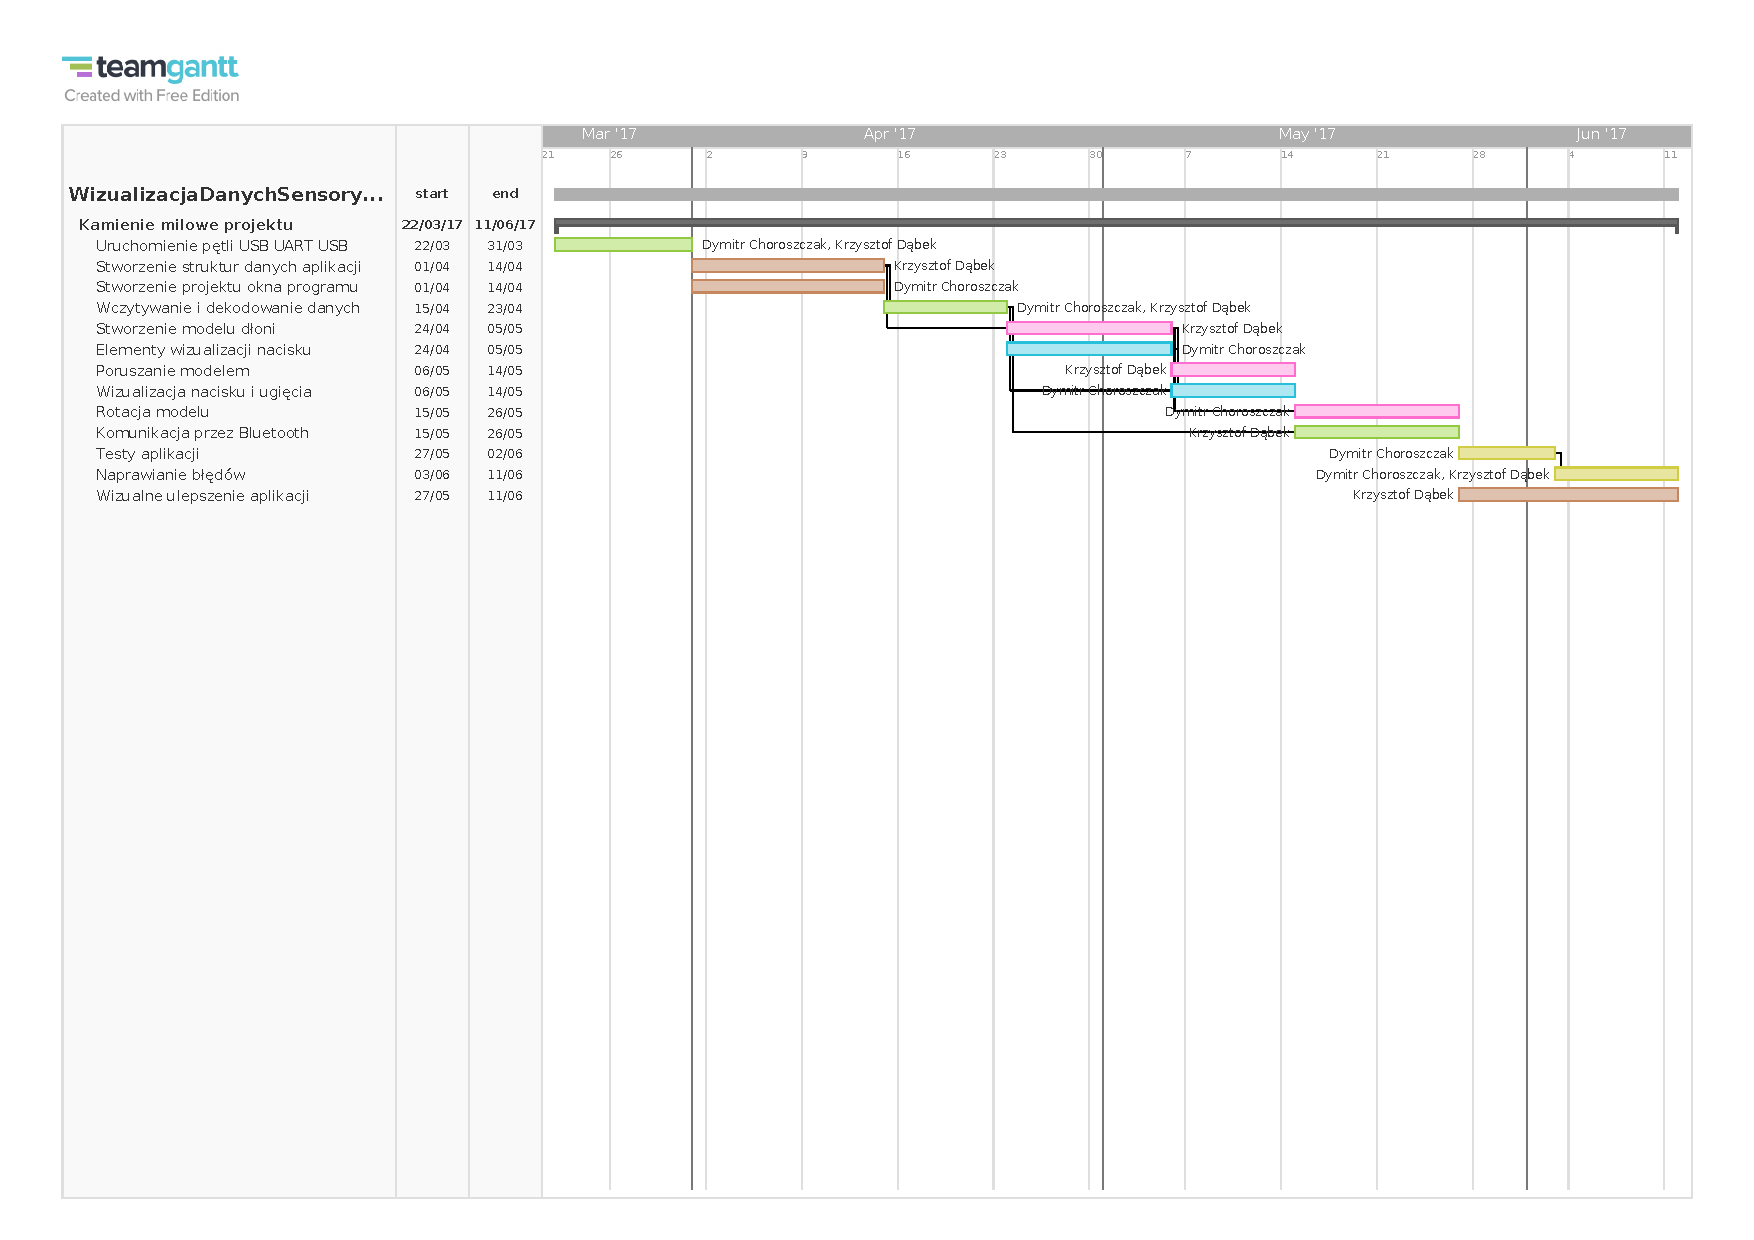
\includepdf[pages={-},angle=90]{Gantt.pdf}

\section{Podsumowanie}
\begin{itemize}
\item Niedokładne odwzorowanie ruchu ręki spowodowane jest trudnościami w przeprowadzeniu dokładnych pomiarów oraz aproksymacji.
\item Pomiary obarczone są dużym błędem z powodu niestabilnej konstrukcji (czujniki przesuwają się) oraz problemu w wyborze metody pomiarowej.
\item Z powodu braku miejsca i zbyt dużej ilości przewodów zrezygnowano z LEDów RGB na rękawicy.
\item Z powodu błędnego funkcjonowania modułu Bluetooth komputera oraz niezadowalającej szybkości przesyłu, zrezygnowano z połączenia rękawicy.
\item Przygotowana aplikacja umożliwia wizualizację danych rękawicy oraz analizę danych pod względem wykrywania gestów.
\item Zrezygnowano z parametryzacji odczytów akcelerometru do kątów RPY (ograniczono się do kąta Pitch) z powodu dużych błędów w obliczaniu kątów oraz niestabilności danych z akcelerometru.
\item Zrezygnowano z części interfejsu użytkownika z powodu ograniczeń czasowych lub zbytniego skomplikowania założonej funkcji. Najważniejsze funkcje zostały zaimplementowane zgodnie z założeniami projektu.
\end{itemize}

\end{document}